\def\year{2019}\relax
%File: formatting-instruction.tex
\documentclass[letterpaper]{article} %DO NOT CHANGE THIS
\usepackage{aaai19}  %Required
\usepackage{times}  %Required
\usepackage{helvet}  %Required
\usepackage{courier}  %Required
\usepackage{url}  %Required
\usepackage{graphicx}  %Required
\usepackage{color, amssymb, multirow, algorithm, inputenc, algpseudocode, amsmath}  % Yerong Customized
\DeclareMathOperator{\Tr}{Tr} % Yerong Customized
\frenchspacing  %Required
\setlength{\pdfpagewidth}{8.5in}  %Required
\setlength{\pdfpageheight}{11in}  %Required
%PDF Info Is Required:
\pdfinfo{
Provable word embedding for the skip-gram word2vec model}
\setcounter{secnumdepth}{0}
\begin{document}
% The file aaai.sty is the style file for AAAI Press 
% proceedings, working notes, and technical reports.
%

\title{Provable word embedding for the skip-gram word2vec model}

\author{Anonymous}

\maketitle

\begin{abstract}
To be written
\end{abstract}

(In \textcolor{magenta}{magenta color} is our comments to drive the writing; in plain black color will be our text)

\section{Introduction}
\textcolor{magenta}{What is the problem we focus on? Word-embedding, why it is important, where it is used, some references from public science \& media showing its significance.}

\textcolor{magenta}{What is the current state of the art \& what are the shortcomings? Here, we should describe how people solve this problem, what are the tools they use (SGD, Riemannian, etc.) and what are the problems with these methods. We shouldn't spend that much space on related work as there will be a Related Work section next.}

\textcolor{magenta}{What is our perspective? Computational. We need to stress out that we do not focus on finding a better linguistic metric, but given word2vec model interpretation as matrix factorization, we identify the problems of using classical methods that involve huge matrix manipulations, and we propose alternatives. At the same time, we are interested in proposing theory that justifies partially what we observe in practice. E.g., here we should say that current approaches are expensive computationally, as well as non-convex with no theory.}

Word embedding represents one of the most successful applications of unsupervised learning. It has shown geralization power in varities of NLP tasks, part-of-speech tagging \cite{abka2016evaluating}, document level metric learning\cite{kusner2015word}, machine translation \cite{NIPS2013_5021}\cite{zou2013bilingual} etc.

In this paper, we train Skip-Gram model with negative sampling (SGND) under the framework of Bi-factorized gradient descent (BFGD). We show that with BFGD, which does not require singular value decomposition at each iteration, we can obtain similar liguistic performance compared to Splitting Projection Algorithm. And BFGD is able to train the model efficiently as the size of a corpus goes up, since it does not require singular value decomposition at each iteration.
As we will see, with update rule in word2vec a special version of stochastic gradient descent under BFGD framework, this discussion opens a critical topic on how to train SGNS both efficiently and effectively --- how to design a good stochastic/batched version of BFGD and train Skip-Gram model without loss of performance.
\textcolor{magenta}{What are our contributions? We need to write them down in bullets; this will be written after we have all the rest}.

\section{Background \& Related Work}
\textcolor{magenta}{Set up the problem: notation + mathematical description}
\textcolor{magenta}{What are the works before us: a more detailed description. What did they contribute, how did they evolve the field?}

\textcolor{magenta}{What questions are still open?}


The Skip-Gram model is introduced in \cite{NIPS2013_5021}, which assumes a corpus of words $w_1$, $w_2$ ... $w_n$ and correponding contexts. For every individual word $w_i$, a context $c$ is defined as a word within a $L-$sided window surrounding it, i.e. $w_{i-L},\cdots, w_{i-1},w_{i+1},\cdots,w_L$. Following notations in \cite{levy2014neural}, we denote $\#(w,c)$ as number of word-context pairs and $\#(w)$ are abbreviation for
\begin{equation}
\#(w)=\sum_{c'}\#(w,c'),\quad\#(c)=\sum_{w'}\#(w',c)	
\end{equation}

It is also convenient to define the set of observed word-context pairs as $D$, and $|D|=\sum_{w,c}\#(w,c)$


The negative sampling takes a word-context pair and samples $k$ negative pairs $(w,c_N)$ aligning with it, where $k$ is a hyperparameter and equals $5$ in experiments. In every negative pairs, the context is generated from the context distribution from the corpus, which is:
\begin{equation}
	c_N\sim P_D(c)=\frac{\#(c)}{|D|}\footnote{In word2vec implementation, $c_N\sim P_D(c)=\frac{\#(c)^{3/4}}{|D|}$, but in mathematics view SGNS is still doing factorization}
\end{equation}
Therefore for every word-context pair in vocabulary, the SGNS objective is:
\begin{equation}
	l_{SGNS}(w,c)= \#(w,c)\log[\sigma(w^\top c)]+k\cdot\mathbb{E}_{c_N\sim P_D}\log[\sigma(-w^\top c_N)]
\end{equation}
When the online learning goes through all word-context pairs in corpus, SGNS model learns distributed word representation by maximizing the following objective function:
\begin{equation}
	\max_{w,c} \sum_{w,c}\#(w,c)\log\sigma(w^\top c)+k\cdot\mathbb{E}_{c_N\sim P_D}[\log \sigma(-w^\top c_N)] \label{eq: original SGNS}
\end{equation}
\subsection{Matrix Factorization}
As what is commonly accepted in literature, some of the "simplest" word embedding models can be viewed as matrix factorizations \cite{li2015word}\cite{NIPS2013_5021}: SGNS is factorizing \textit{shifted} Pointwise Mutual Information matrix, Noise-Contrastive Estimation \cite{gutmann2010noise} is factorizing \textit{shifted} log-conditional-probability matrix for instance. Despite different views on the contrary\cite{arora2015rand}, it has been of parculiar interests to view word embedding views as matrix factorization and studying the landscape of those objectives \cite{li2015word}\cite{mimno2017strange}.
\subsection{Project-Splitting algorithm on SGNS}
On \cite{fonarev2017riemannian} illustrates a general two-step scheme for training SGNS word embedding model and suggested a search of a solution in the low-rank form via Riemannian optimization framework.
\subsection{Linguistic scores}

\section{Our approach}
\textcolor{magenta}{Description of the algorithm, details and discussion on initialization + step size, maybe already here have some plots to show how these behave (without giving away comparison results, just showing what is their trend in}

In this paper, we follow literature dicussions characterizing SGNS as a matrix factorization problem \cite{levy2014neural}\cite{levy2015improving}. The expectation term $\mathbb{E}_{c_N\sim P_D}[\log \sigma(-w^\top c_N)]$ can be explicitly expressed as:
\begin{equation}
	\mathbb{E}_{c_N\sim P_D}[\log \sigma(-w^\top c_N)]=\sum_{c_N}\frac{\#(c_N)}{|D|}\log{\sigma(-w^\top c_N)}
\end{equation}
And one can show that SGNS objective \ref{eq: original SGNS} is factorizing the following matrix \cite{levy2014neural}:
\begin{equation}
	X=W^\top C= PMI(w_i, c_j)-\log k \label{eq: SPPMI}
\end{equation}
where columns in $W$ and $C$ are $w_i$ and $c_i$ respectively. And in our setting, the vocabulary size is $V$ , and the hidden layer size is $d$, so both $W$ and $C$ are $d\times V$.

Different from projector-splitting scheme\cite{fonarev2017riemannian} which shows advantages in optimizing a low-rank $X$ on SGNS model, we observed that the matrix form SGNS objective is both smooth and convex in $X$. And with the explicit expression of SGNS objective $L_{SGNS}(X)$:
\begin{equation}
	L_{SGNS}(X)=\sum_{w,c}\{\#(w,c)\log\sigma(w^\top c)+k\cdot\sum_{c_N}\frac{\#(c_N)}{|D|}[\log \sigma(-w^\top c_N)]\} \label{eq: smoothness}
\end{equation}
$L_{SGNS}(X)$ is $L-$smooth with Lipschitz constant $$L=\frac{1}{4}\|\{\#(w,c)+k\frac{\#(w)\#(c)}{|D|}\}_{w,c}\|_F$$



Then we can borrow ideas from Bi-factorized gradient descent  \cite{park2016finding}

\begin{algorithm}
\caption{BFGD on Skip-Gram Model with Negative Sampling}\label{alg:bfgd}
\begin{algorithmic}[1]
\Procedure{BFGD}{$W_0,C_0, \eta, K$} \Comment{$W_0,C_0$ are initial encoding and decoding matrices, $\eta$ is the step size and $K$ is the total number of iterations}
\State $W\gets W_0$
\State $C\gets C_0$
\For{$i\gets 1, \cdots, K$}
	\State{Calculate gradient of loss $\nabla L(W^\top C)$}
	\State{$W\gets W+\eta\cdot C\nabla L(W^\top C)$}
	\State{$C\gets C+\eta\cdot W\nabla L(W^\top C)^\top$}
\EndFor
\State \textbf{return W, C}
\EndProcedure
\end{algorithmic}
\end{algorithm}
In the BFGD agorlithm \ref{alg:bfgd}, the complexity for each iterations is $O(V^2d)$: with hidden dimension fixed, the running time scales quadratically with the size of the vocabulary. As a comparision, Project-Splitting\cite{fonarev2017riemannian} operates QR factorization in updating parameters and requires $O(V^3)$ unit operations at each iteration. And in experiments, our see our approach is at least two times faster than the Project-Splitting scheme.

\textcolor{magenta}{Here, we should have a figure with the algorithm's steps etc.}

\section{Experimental results}
\textcolor{magenta}{We will move a bit unconventionally and show first some experimental results: this is what we are currently working on}
\paragraph{Experimental Settings} In experiments, we trained skip-gram negative sampling with Bi-Factorized gradient descent on two corpora:  "enwik9" corpus \cite{mahoney2011large} and New York Times corpus (NYT) \cite{sandhaus2008new}. The "enwik9" contains the first billions bytes of the Wikipedia dump on Mar. 3, 2006. We ignore words that appear less than 100 times in this dump and train a model with vocabulary size 37,360. The New York Times Annotated Corpus contains over a million articles tagged with metadata. These articles are published between 1987 and 2007. We pick articles from 2000 to 2005 for training.  We preprocessed the data with Stanford CoreNLP tookenizer \cite{manning2014stanford}. It has 13,567,603 sentences and we use a dictionary of the 40,000 most frequent words from this subcorpus.

In order to reduce training noise from frequent words: we do subsampling and ignore a word $w$ in a sentence with a probability
\begin{equation}
P(f(w))= 1-(\sqrt{\frac{f(w)}{t}}+1)\cdot\frac{t}{f(w)}\label{eq:subsampling}
\end{equation}
where where $t$, $f(w)$ are subsampling threshold and the frequency of the word respectively. We have to point out equation \ref{eq:subsampling} is used in word2vec\footnote{https://code.google.com/archive/p/word2vec} and is an adapted version of subsampling in \cite{NIPS2013_5021}.
\subsection{Evaluation}
We illustrate equivalence of BFGD and PS analogy tasks and similarity tasks.
\paragraph{Analogy} The analogy test datasets come from Google analogy \cite{NIPS2013_5021} and MSR's analogy dataset \cite{mikolov2013linguistic}.  Google’s analogy dataset  contains 19,544 questions of two types --- semantic and syntatic analogies. Semantic questions are analogies in semantic sense, as ``Greece  is to Athens as Iraq is to Baghdad'', whereas syntactic questions are related to tokens and their syntactic variants, as ``amazingly is to amazing as apparently is to apparent''. MSR's analogy test set has 8,000 morpho-syntactic analogy questions. it is composed of the syntactic kind of tasks.
\begin{table}[]
\begin{tabular}{|c|c|c|c|c|c|c|c|}
\hline
   dim      &      & sem & syn & wordsim & men & simlex & murk \\ \hline

\multirow{3}{*}{100} & SGD   &     &     &         &     &        &      \\ \cline{2-8} 
					 & PS   &     &     &         &     &        &      \\ \cline{2-8} 
                     & BFGD &     &     &         &     &        &      \\ \hline
\multirow{3}{*}{300} & SGD   &     &     &         &     &        &      \\ \cline{2-8} 
					 & PS   &     &     &         &     &        &      \\ \cline{2-8} 
                     & BFGD &     &     &         &     &        &      \\ \hline
\multirow{3}{*}{300} & SGD   &     &     &         &     &        &      \\ \cline{2-8} 
					 & PS   &     &     &         &     &        &      \\ \cline{2-8} 
                     & BFGD &     &     &         &     &        &      \\
\hline
\end{tabular}
\caption{Comparison of different methods on liguistic scores, on different dimensions}
\end{table}
\begin{table}[]
\begin{tabular}{|c|c|c|c|c|c|c|c|}
\hline
   dataset  &      & sem & syn & wordsim & men & simlex & murk \\ \hline

\multirow{3}{*}{NYT} & SGD   &     &     &         &     &        &      \\ \cline{2-8} 
					 & PS   &     &     &         &     &        &      \\ \cline{2-8} 
                     & BFGD &     &     &         &     &        &      \\ \hline
\multirow{3}{*}{enwik} & SGD   &     &     &         &     &        &      \\ \cline{2-8} 
					 & PS   &     &     &         &     &        &      \\ \cline{2-8} 
                     & BFGD &     &     &         &     &        &      \\ \hline
\end{tabular}
\caption{Comparison of different methods on liguistic scores, on different dataset, we kept dimension $d=300$}
\end{table}
\begin{figure}
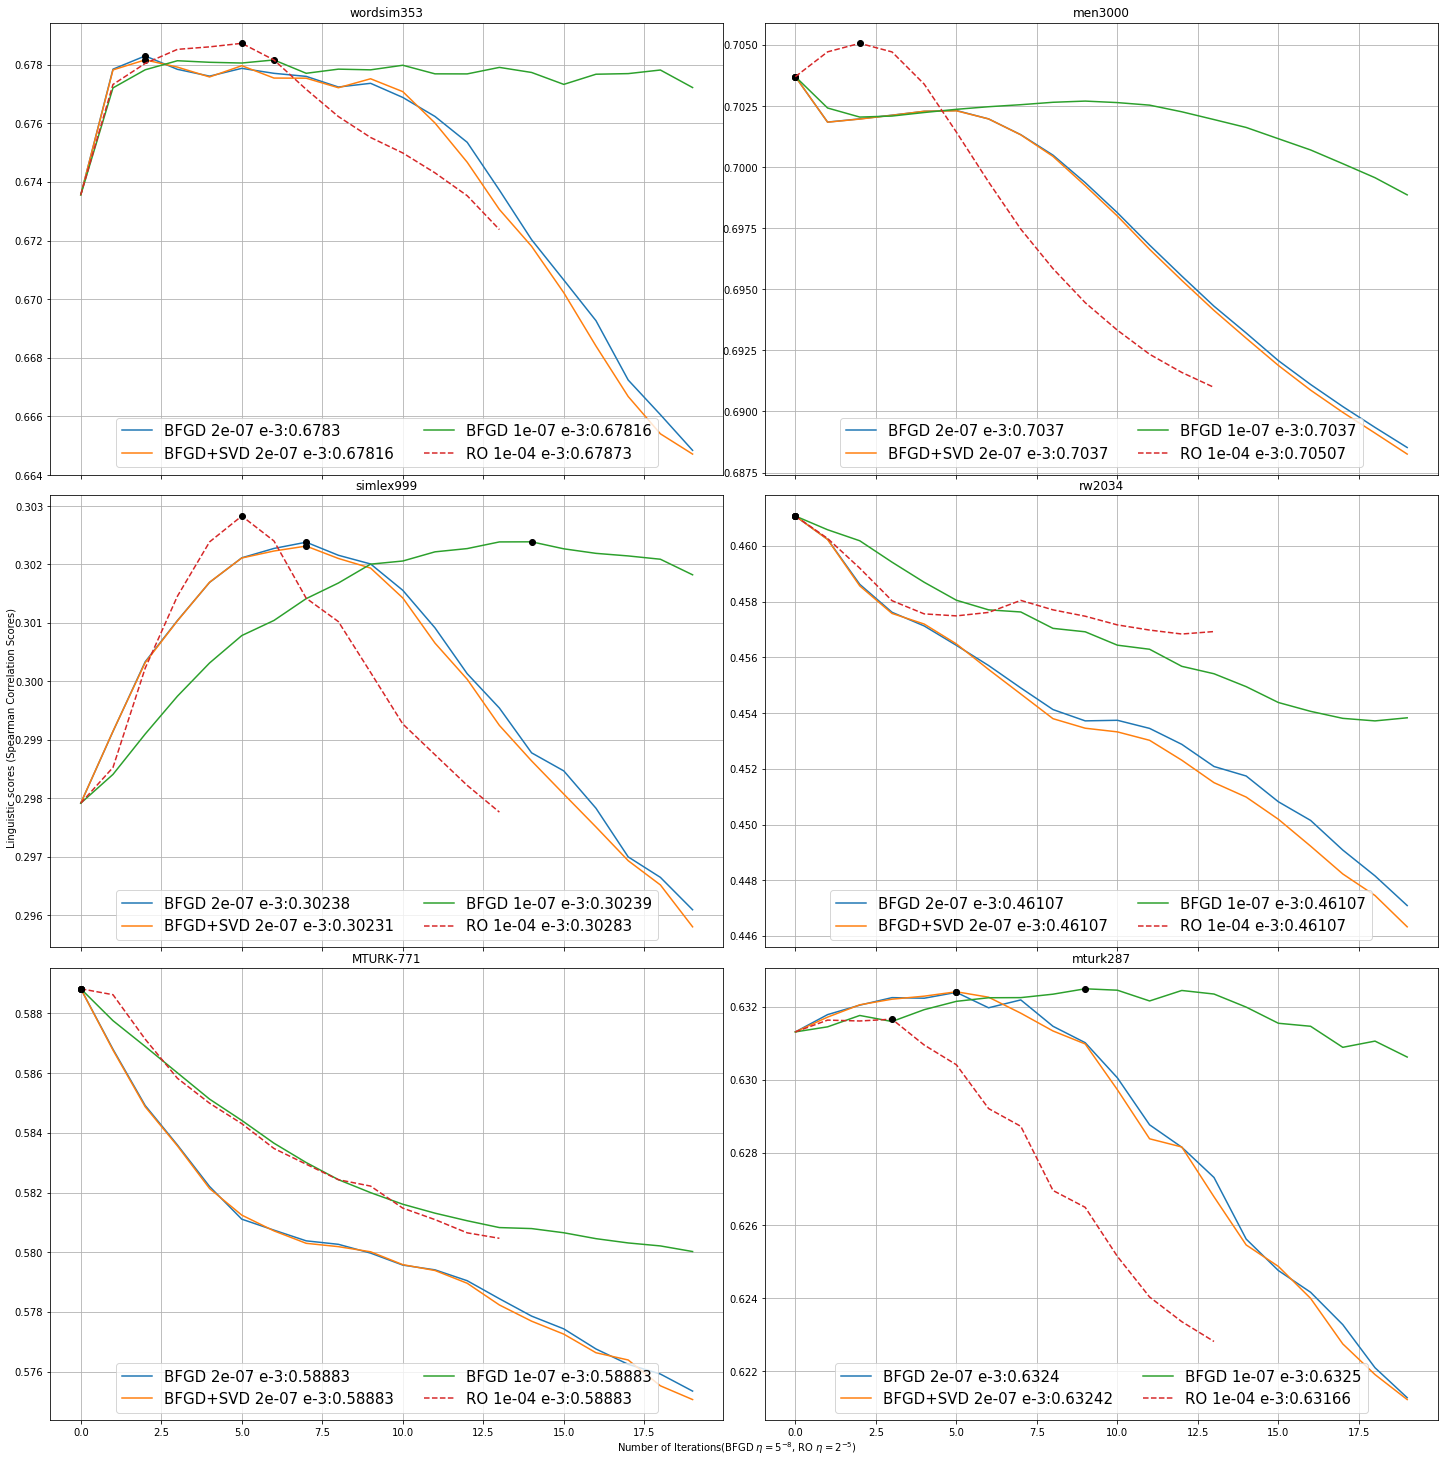
\includegraphics[width=\linewidth]{img/correlation.png} 
\end{figure}
\section{Theoretical guarantees}
\textcolor{magenta}{This is where we will try to focus on after we have fixed the experiments. 
\begin{itemize}
\item What are the properties of the objective?
\item What is known out there w.r.t. theory? What can we reuse for our algorithm?
\item Initialization: what can we say about it? Any theory?
\item Are there local minima for the non-convex problem we have?
\item what about the stochastic version? SVRG version? Are there prior results on this?
\item Can we use momentum/acceleration? Can we gain theoretically?
\end{itemize}}
In this section, we provide theoretical guarantees for the convergence of BFGD algorithm. As shown in analysis above, SGNS objective $L_\text{SGNS}$ is smooth as well as strictly convex, we focus our discussions based on this setting.

Since BFGD gives the best results starting from SPPMI matrix, we provide a convergence guarantee for SPPMI initialization.

From matrix factorization on SGNS objective \cite{levy2014neural} sparse SPPMI matrix and dense PPMI matrix. PPMI is $X^*$, the optimal solution for SGNS. SPPMI is the $X^0$, with its rank$-r$ approximation $X_r^0=W_0^\top C_0$ the starting point.

From defintion of SPPMI and PPMI matrix we have
%\begin{equation}
%\|X^0-X^*\|_F\le\|X^0|_F\le\|X^*|_F
%\end{equation}
%From triangle and Mirsky's theorem, we have
%\begin{equation}
%\begin{split}
%\|X^0-W_0^\topC_0\|_F\le\|X^*-X_r^*\|_F+\|X^0-X_r^*\|%_F\\
%\end{split}
%\end{equation}
%Thus,
%\begin{equation}
%\|X_r^*-W_0^\topC\|_F\le\|X^0-X^*\|_F+\|X^*-X_r^*\|_F+%\|X^0-W_0^\topC_0\|_F\cite{park2016finding}
%\end{equation}
%\begin{equation}
%\|X^*-W_0^\topC\|_F\le\|X^0-X^*\|_F+\|X^*-X_r^*\|_F+\|X^0-X_r^*\|_F
%\end{equation}
Assume for any number of rows in $X$, $L-smoothness$ holds.
\subsection{FGD}
On one iteration $X$ is $V \times V$:
$$U^+=U-\eta (\nabla f(X)U)^i= U-\eta (\nabla f)^iU=U-\eta\begin{bmatrix}
    0 \\
    0 \\
    %\hdotsfor{1} \\
	(\nabla f)_iU\\    
    0 
\end{bmatrix}$$

Here $\nabla f$ is a shorthand for $\nabla f(X)$ and $\eta$ is given by
\[
\eta=\frac{1}{16(L\|X^0\|_2+\|\nabla f(X^0)\|_2)}
\]
 We are using $(\nabla f)^i$ for the full $V\times V$ matrix and $(\nabla f)_i$ for a random component/row:

$$(\nabla f)^i=\begin{bmatrix}
0 \\
0 \\
%\hdotsfor{1} \\
(\nabla f)_i\\    
0 
\end{bmatrix}$$


For simplification, we define $\Lambda=I-\frac{\eta}{2}Q_UQ_U^\top(\nabla f(X))^i$, which corresponds to the stochastic gradient $(f(X))^i$. It is easy to check that 
\begin{equation}
X^+=X-\eta(\nabla f(X))^iX\Lambda-\eta\Lambda^\top X(\nabla f(X))^i
\end{equation}
For the randomly picked $i$ we have:
%\begin{equation}
%\begin{split}
%f(X^+)-f(X)&\le\langle\nabla f, X^+-X\rangle+\frac{L}{2}\|X^+-X\|_F^2\\
%&=-\eta\langle(\nabla f)_i, (\nabla f)_i\rangle+\frac{L}{2}\|X^+-X\|_F^2\\
%&=-\eta\langle\nabla_i f, \nabla_i f\rangle+\frac{L}{2}\|X^+-X\|_F^2\\
%&=\langle\nabla_i f, X^+-X\rangle+\frac{L}{2}\|X^+-X\|_F^2
%\end{split}
%\end{equation}

%This follows from the symmetry of $X$, $f(X)$ the observation: $$\Tr(\nabla^\top f\Lambda^\top X(\nabla f)^i)=\Tr(\Lambda^\top X(\nabla f)^i\nabla^\top f)=\Tr(\nabla f(\nabla^\top  f)^i X\Lambda)$$
\begin{equation}
	\begin{split}
		&\Tr(\nabla^\top f(\nabla f)^iX\Lambda)\\
		=&\Tr(
		\begin{bmatrix}
		\cdots(\nabla f)^\top_i\cdots 
		\end{bmatrix}
		\begin{bmatrix}
			0 \\0 \\(\nabla f)_i\\	0 
		\end{bmatrix}X\Lambda)\\
	\end{split}
\end{equation}
%		=&\Tr( (\nabla^\top f)_i(\nabla f)_i X\Lambda)\\
%=&\Tr( (\nabla^\top f)_i(\nabla f)_i UU^\top)-\Tr( (\nabla^\top f)_i(\nabla f)_i UU^\top Q_UQ^\top_U(\nabla f)^i)\\
%=&\Tr( (\nabla f)^i(\nabla f)^i UU^\top)-\Tr( (\nabla f)^i(\nabla f)^i UU^\top Q_UQ^\top_U(\nabla f)^i)\\
%\ge& (1-\frac{\eta}{2}\|Q_UQ_U^\top\|_2)\|\nabla f U\|_f^2

\begin{equation}
	\begin{split}
		&\Tr(\nabla^\top f\Lambda^\top X(\nabla f)^i)\\
		=&\Tr((\nabla f)^i\nabla^\top f\Lambda^\top X)\\
		=&\Tr(
		\begin{bmatrix}
			0 \\0 \\(\nabla f)_i\\0 
		\end{bmatrix}
		\begin{bmatrix}
			\cdots(\nabla f)^\top_i\cdots 
		\end{bmatrix}\Lambda^\top X)
	\end{split}
\end{equation}

Thus 
\begin{equation}
\begin{split}
&\mathbb{E}[\Tr(\nabla^\top f\Lambda^\top X(\nabla f)^i)]=\mathbb{E}[\Tr(\nabla^\top f\Lambda^\top X(\nabla f)^i)]\\
&=\frac{1}{V} \Tr(\nabla f(X)\nabla f(X)X\Lambda)
\end{split}
\end{equation}
Conditioned on $X$, we have
\begin{equation}
\begin{split}
&\mathbb{E}[f(X^+)]-f(X)\\&\le \mathbb{E}[\langle\nabla_i f, X^+-X \rangle]+\frac{L}{2}\mathbb{E}[\|X^+-X\|_F^2] \\
&=-\frac{2\eta}{V}\Tr(\nabla f(X)\nabla f(X)X\Lambda)+\frac{L\eta^2}{2V}\|\nabla f(X)X\Lambda+\nabla \Lambda Xf(X)\|^2_F\\
&\overset{(i)}{\le}-\frac{2\eta}{V}\Tr(\nabla f(X)\nabla f(X)X\Lambda)+\frac{2L\eta^2}{V}\|\nabla f(X)X\Lambda\|^2_F\\
&\le-\frac{2\eta}{V}\Tr(\nabla f(X)\nabla f(X)X\Lambda)+\frac{2L\eta^2}{V}\|\nabla f(X)U\|^2_F\|X\|_2\|\Lambda\|^2_2\\
&\overset{(ii)}{\le}-\frac{2\eta}{V}\Tr(\nabla f(X)\nabla f(X)X\Lambda)+\frac{\eta}{7V}(\frac{33}{32})^2\|\nabla f(X)U\|^2_F\\
&\overset{(iii)}{\le}-\frac{31\eta}{16V}\|\nabla f(X)U\|^2_F+\frac{\eta}{7V}(\frac{33}{32})^2\|\nabla f(X)U\|^2_F\\
&\le-\frac{17\eta}{10V}\|\nabla f(X)U\|^2_F
\end{split}
\end{equation}
$(i)$ is from triangle inequality, $(ii)$ is from equation (18) in \cite{park2016finding} and $(iii)$ is from Lemma $A.5$ in \cite{park2016finding} which implies $\|\Lambda\|_2\le \frac{33}{32}$ and $\sigma_V(\Lambda)\ge \frac{31}{32}$.

Which is to say for the optimal $X_r^*$:
\begin{equation}
 \mathbb{E}[f(X^+)]-f(X_r^*)\le f(X)-f(X_r^*)-\frac{17\eta}{10V}\|\nabla f(X)U\|^2_F
\label{eq: sublinear}
\end{equation}
By equation(18) in \cite{tu2015low} we have 
\begin{equation}
f(X)-f(X_r^*)\le\frac{5}{2}\|\nabla f(X)\|_F\text{DIST}(U,U^*_r) \label{eq:distance}
\end{equation}
Thus with 
$$\delta^+= \mathbb{E}[f(X^+)]-f(X_r^*)\quad \delta=\mathbb{E}[f(X)]-f(X_r^*)$$
%\end{equation}
We can easily see
\begin{equation}
\begin{split}
\delta^+&\le\delta -\frac{17\eta}{10V}\|\nabla f(X)U\|^2_F\\
&\le\delta -\frac{17\eta}{10V}\times(\frac{2}{5})^2\cdot\frac{\delta^2}{\text{DIST}^2(U,U^*_r)}\\
\end{split}
\end{equation}
\begin{equation}
\frac{1}{\delta^+}\le\frac{1}{\delta}+ \frac{\eta}{5V\cdot\text{DIST}(U,U^*_r)}\\
\end{equation}
\subsection{Convergence of Word Embedding}
Define $U=\begin{bmatrix}W\\C\end{bmatrix}$, $X=WC^T$
\begin{equation}
\nabla_U f=\begin{bmatrix}\nabla_X fC\\\nabla^T_X fW\end{bmatrix}=\begin{bmatrix}0&\nabla_X f\\ \\\nabla^T_X f&0\end{bmatrix}\begin{bmatrix}W\\C\end{bmatrix}\label{eq: gradient}
\end{equation}
Specifically, 
\begin{equation}
\begin{split}
	&\{\nabla_X f(X=WC^T)\}_{kl}\\
	=&\sum_{i'}\sum_{j'}\#(w_k, c_l)\cdot(\sigma(-c_lw^T_k))+k\sum_{i'}\#(w_{i'}, c_l)\cdot(-\sigma(c_lw^T_k))\label{eq: grad f}
\end{split}
\end{equation}
Going back to the skip gram iterations, which can be seen as updating the matrix $U$.

Assume from $U$ to $U^+$, we observed a word-context pair $(w_i,c_j)$ with $k$ negative samples oriented to the oriented word $w_i$, namely $(w_i,c_{n1}),\cdots,(w_i,c_{nk})$, Define matrix gradient matrix $G$ as follows:
\begin{equation}
G=\begin{bmatrix}0&G'\\G'^T&0\end{bmatrix}
\end{equation}
where
\begin{equation}
\begin{split}
\{G'\}_{i,j}&=\sigma(-c_jw_i^T)\\
\{G'\}_{i,n1}&=-\sigma(c_{n1}w_i^T)\\
\cdots\\
\{G'\}_{i,nk}&=-\sigma(c_{nk}w_i^T)
\end{split}
\end{equation}


with other elements in $G'$ zeros;

%\[
%\begin{split}
%\{G_n\}_{j,i}&=-\sigma(-c_jw_i^T)\\
%\{G_n\}_{n1,i}&=\sigma(c_{n1}w_i^T)\\
%\cdots\\
%\{G_n\}_{nk,i}&=\sigma(c_{nk}w_i^T)\\
%\end{split}
%\]

Therefore in matrix form, $U$ is updating to $U^+$ with gradient matrix $G$:
\begin{equation}
U^+=U+\eta GU \label{eq: ascent}
\end{equation}
Intuitively, $G'$ is updating $\nabla_X f$ row by row.

We have to show $G$ is doing coordinate ascend:

\textbf{Lemma:}  Intuitively, $G'$ is updating $\nabla_X f$ row by row, specifically,
\begin{equation}
	\mathbb{E}(G')=\frac{1}{\sum_{i'}\sum_{j'} \#(w_{i'}, c_{j'})}\cdot \nabla_X f
\end{equation}

\textbf{Proof:} In one epoch, as the observed pairs go through all corpus, $(w_i,c_j)$ appears with distribution: \[\{G'\}_{i,j}\sim\frac{\#(w_i, c_j)}{\sum_{i'}\sum_{j'} \#(w_{i'}, c_{j'})}\]
with negative samples from the distribution:
 \[\{G'\}_{i,ns}\sim\frac{\sum_{i'}\#(w_{i'}, c_{ns})}{\sum_{i'}\sum_{j'} \#(w_{i'}, c_{j'})}\quad\text{which is independent of $i$}\]
 
 Thus, for an individual element $\{G'\}_{k,l}$ in $G'$, we have
 \[
 \begin{split}
&\mathbb{E}(\{G'\}_{k,l})\\
=&\sum_{i'}\sum_{j'}\frac{\#(w_k, c_l)}{\sum_{i'}\sum_{j'} \#(w_{i'}, c_{j'})}\cdot(\sigma(-c_lw^T_k))+\frac{k\sum_{i'}\#(w_{i'}, c_{ns})}{\sum_{i'}\sum_{j'} \#(w_{i'}, c_{j'})}\cdot(-\sigma(c_lw^T_k))\\
=&\frac{1}{\sum_{i'}\sum_{j'} \#(w_{i'}, c_{j'})}[\sum_{i'}\sum_{j'}\#(w_k, c_l)\cdot(\sigma(-c_lw^T_k))+k\sum_{i'}\#(w_{i'}, c_{ns})\cdot(-\sigma(c_lw^T_k))]
 \end{split} \label{eq :expectation}\]
  
Matching \ref{eq :expectation} with \ref{eq: grad f}, we know that
\begin{equation}
\mathbb{E}(\{G'\}_{k,l})=\frac{1}{\sum_{i'}\sum_{j'} \#(w_{i'}, c_{j'})}\cdot \{\nabla_X f(X=WC^T)\}_{kl} \label{eq: scaling}
\end{equation} 
\[
\text{Q.E.D}\blacksquare
\]
This lemma tells us that 
\begin{equation}
a
\end{equation}
For short, we denote the scaling factor as:
\begin{equation}
S={\sum_{i'}\sum_{j'} \#(w_{i'}, c_{j'})}
\end{equation}
Defining define $\Lambda=I-\frac{\eta}{2}Q_UQ_U^\top G$, from equation \ref{eq: ascent}, we know
\begin{equation}
X^+=\begin{bmatrix}W^+\\C^+\end{bmatrix}\begin{bmatrix}W^{+T}C^{+T}\end{bmatrix}=X+\eta GX\Lambda+\eta\Lambda^\top XG
\end{equation}
The loss function $f(X)$ is concave on $X=\begin{bmatrix}W\\C\end{bmatrix}\begin{bmatrix}W^{T} C^{T}\end{bmatrix}$ and $L'=\frac{L}{2}-$ smooth with $L$ in equation \ref{eq: smoothness}
\
Conditioned on $X$, we have
\begin{equation}
\begin{split}
&\mathbb{E}[f(X^+)]-f(X)\\&\ge \mathbb{E}[\langle \nabla f(X), X^+-X \rangle]-\frac{L'}{2}\mathbb{E}[\|X^+-X\|_F^2] \\
&=\frac{2\eta}{S}\Tr(\nabla f(X)\nabla f(X)X\Lambda)-\frac{L'\eta^2}{2S}\|\nabla f(X)X\Lambda+\nabla \Lambda Xf(X)\|^2_F\\
&\overset{(i)}{\ge}\frac{2\eta}{S}\Tr(\nabla f(X)\nabla f(X)X\Lambda)-\frac{2L'\eta^2}{S}\|\nabla f(X)X\Lambda\|^2_F\\
&\ge\frac{2\eta}{S}\Tr(\nabla f(X)\nabla f(X)X\Lambda)-\frac{2L'\eta^2}{S}\|\nabla f(X)U\|^2_F\|X\|_2\|\Lambda\|^2_2\\
&\overset{(ii)}{\ge}\frac{2\eta}{S}\Tr(\nabla f(X)\nabla f(X)X\Lambda)-\frac{\eta}{7S}(\frac{33}{32})^2\|\nabla f(X)U\|^2_F\\
&\overset{(iii)}{\ge}\frac{31\eta}{16S}\|\nabla f(X)U\|^2_F-\frac{\eta}{7S}(\frac{33}{32})^2\|\nabla f(X)U\|^2_F\\
&\ge\frac{17\eta}{10S}\|\nabla f(X)U\|^2_F
\end{split}
\end{equation}

$(i)$ is from triangle inequality, $(ii)$ is from equation (18) in \cite{park2016finding} and $(iii)$ is from Lemma $A.5$ in \cite{park2016finding} which implies $\|\Lambda\|_2\le \frac{33}{32}$ and $\sigma_V(\Lambda)\ge \frac{31}{32}$

Due to concaveness of $f(X)$ on $X$ and definition of $\text{DIST}(\cdot,\cdot)$, we have 

\section{Conclusions}
\textcolor{magenta}{In discussion, we should claim that our purpose is to design a distributed version of the non-convex algorithm that can scale up and out.}
 
%References and End of Paper
%These lines must be placed at the end of your paper
\bibliography{refs.bib}
\bibliographystyle{aaai}

\end{document}
